\documentclass[12pt,a4paper]{article}
\usepackage[utf8]{}
\usepackage[T1]{fontenc}
\title{EP1200 - Datasys anteckningar}
\author{Yunshan Luo}


\renewcommand{\baselinestretch}{0.2}

\setlength{\hoffset}{-18pt}         
\setlength{\oddsidemargin}{0pt} % Marge gauche sur pages impaires
\setlength{\evensidemargin}{0pt} % Marge gauche sur pages paires
\setlength{\marginparwidth}{54pt} % Largeur de note dans la marge
\setlength{\textwidth}{481pt} % Largeur de la zone de texte (17cm)
\setlength{\voffset}{-18pt} % Bon pour DOS
\setlength{\marginparsep}{7pt} % Séparation de la marge
\setlength{\topmargin}{0pt} % Pas de marge en haut
\setlength{\headheight}{13pt} % Haut de page
\setlength{\headsep}{4pt} % Entre le haut de page et le texte
\setlength{\footskip}{27pt} % Bas de page + séparation
\setlength{\textheight}{720pt} % Hauteur de la zone de texte (25cm)

\usepackage{natbib}
\usepackage{graphicx}
\usepackage{amssymb}
\usepackage{amsmath} % Required for the align* environment
\usepackage{float}
\usepackage{pgfplots} 
\usepackage{algorithm}
\usepackage{algpseudocode} % test comment
\usepackage[hidelinks]{hyperref}
\pgfplotsset{compat=1.18}


\begin{document}
\title{DD2421 - Machine Learning}
\maketitle
\section{Lecture 1 -- Introduction}
\begin{itemize}
    \item \textbf{Supervised learning:} Learn mappings from A to B, B was provided by a human
    \item \textbf{Unsupervised learning:} Analyzing unstructured data, no labels provided
\end{itemize}

\section{Lecture 2 -- Decision Trees}
\begin{figure}[H]
    \centering
    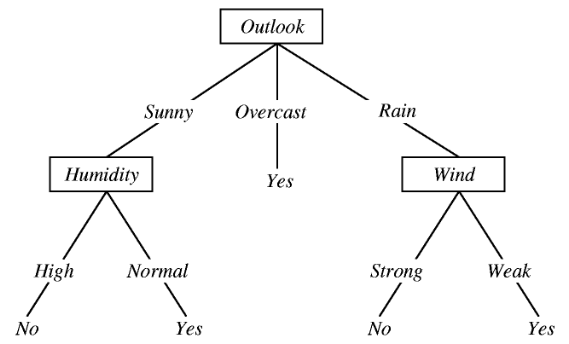
\includegraphics[width=0.75\textwidth]{decision_tree.png}
    \caption{Example of decision tree predicting whether to play tennis based on weather conditions}
    \label{fig:decision_tree}       
\end{figure}

\subsection{How to build a tree}
\begin{enumerate}
    \item Given a set of labeled data
    \item Choose the question with the maximum \textbf{information gain}
    \item \textbf{Terminate} when all data in a node have the same label or when there are no more questions to ask
\end{enumerate}

\subsection{Entropy}
Information gain is measured by:
\[
log_2(\frac{1}{p_i}), \hspace{10pt} p_i = \text{Probability of event }i
\]

\noindent Entropy measures how predictable a dataset is and is defined as:
\[
Entropy = \sum -p_i log_2(p_i)
\]

\subsection{Entropy applied to decision trees}
Ask about the attribute that maximizes the reduction of entropy

% Continue at powerpoint lecture 2, slide 40







\end{document}